\documentclass[12pt,letterpaper]{report}
% Preámbulo compartido para los documentos del Sistema de Solicitudes (UAZ).
% Identidad visual alineada con el SRS. Compilar con pdflatex.
\usepackage[utf8]{inputenc}
\usepackage[T1]{fontenc}
\usepackage[spanish, mexico]{babel}
\usepackage{geometry}
\geometry{left=2.5cm, right=2.5cm, top=2.5cm, bottom=2.5cm}
\usepackage{graphicx}
\usepackage{float}
\usepackage{longtable}
\usepackage{tabularx}
\usepackage{array}
\usepackage{booktabs}
\usepackage{hyperref}
\usepackage{enumitem}
\usepackage{xcolor}
\usepackage{fancyhdr}
\usepackage{titlesec}
\usepackage{caption}
\usepackage{listings}

\definecolor{uazblue}{RGB}{0, 51, 102}
\definecolor{lightgray}{RGB}{240, 240, 240}
\definecolor{codebg}{RGB}{248, 248, 248}

\hypersetup{colorlinks=true, linkcolor=uazblue, urlcolor=uazblue, citecolor=uazblue}

\newcolumntype{L}[1]{>{\raggedright\arraybackslash}p{#1}}
\newcolumntype{C}[1]{>{\centering\arraybackslash}p{#1}}
\newcolumntype{R}[1]{>{\raggedleft\arraybackslash}p{#1}}

\titleformat{\chapter}[display]
  {\normalfont\huge\bfseries\color{uazblue}}{\chaptertitlename\ \thechapter}{20pt}{\Huge}
\titlespacing*{\chapter}{0pt}{-20pt}{40pt}

\lstset{
  basicstyle=\ttfamily\footnotesize,
  backgroundcolor=\color{codebg},
  frame=single,
  rulecolor=\color{lightgray},
  breaklines=true,
  columns=fullflexible,
  showstringspaces=false,
  keepspaces=true,
}

% Portada institucional reutilizable:
% \portada{TÍTULO DEL DOCUMENTO}{Subtítulo opcional}
\newcommand{\portada}[2]{%
\begin{titlepage}
    \centering
    \vspace*{1cm}
    {\Large\bfseries UNIVERSIDAD AUTÓNOMA DE ZACATECAS}\\[12pt]
    {\normalsize UNIDAD ACADÉMICA DE INGENIERÍA ELÉCTRICA}\\[24pt]
    \IfFileExists{uaz.png}{
\includegraphics[width=1.5in]{uaz.png}\\[40pt]}{\vspace{40pt}}
    {\large\bfseries #1}\\[6pt]
    {\large\bfseries SISTEMA DE SOLICITUDES}\\[10pt]
    {\normalsize #2}\\[24pt]
    {\normalsize\bfseries
    Diego Iván Correa Navarrete\\
    Juan Antonio González del Río\\
    Diego Arturo Ramos Ávila\\
    Ángel David Carlos Silva\\}
    \vspace{30pt}
    {\normalsize\bfseries LICENCIATURA EN INGENIERÍA DE SOFTWARE}\\[16pt]
    {\normalsize Junio de 2026}
\end{titlepage}}

\usepackage{pdflscape}
\begin{document}
\portada{ESQUEMA DE BASE DE DATOS}{\mbox{}}
\tableofcontents\newpage

\chapter{Introducción}

Este documento describe el esquema de la base de datos del \textbf{Sistema de
Solicitudes} de la Universidad Autónoma de Zacatecas (UAZ). Comprende el
diagrama entidad-relación, el diccionario de datos por entidad y la
especificación de las relaciones e integridad referencial. La información aquí
contenida se obtuvo mediante introspección directa del esquema de modelos de
Django en ejecución, complementada con la lectura de las definiciones de modelo
del código fuente.

\section{Motor de base de datos}

El sistema emplea \textbf{PostgreSQL} como motor de base de datos en los
entornos productivo y de pruebas, y \textbf{SQLite} en el entorno de desarrollo
local. Toda la interacción con la base de datos se realiza a través del ORM de
\textbf{Django 5.x}; el acceso a la persistencia está contenido en la capa de
repositorios, conforme a la arquitectura Vista $\rightarrow$ Servicio
$\rightarrow$ Repositorio del proyecto.

Algunas características del esquema dependen de PostgreSQL. En particular, los
\emph{índices únicos parciales} (índices con condición \texttt{WHERE}) que
imponen invariantes como ``un solo periodo de mentoría activo por matrícula'' o
``un solo comprobante por solicitud'' requieren PostgreSQL para aplicarse
correctamente.

\section{Convenciones}

\begin{itemize}[leftmargin=1.4em]
  \item \textbf{Nombres de tabla.} Siguen la convención de Django
        \texttt{<app>\_<modelo>} en minúsculas (p.\,ej.
        \texttt{solicitudes\_solicitud}).
  \item \textbf{Llaves primarias.} La mayoría de las entidades usan
        \texttt{UUID} como llave primaria (campo \texttt{id}). Tres entidades
        usan llaves primarias naturales o de negocio:
        \texttt{User.matricula} (matrícula institucional),
        \texttt{Solicitud.folio} (folio legible \texttt{SOL-AAAA-NNNNN}) y
        \texttt{FolioCounter.year} (año). Dos entidades de bitácora
        (\texttt{HistorialEstado}, \texttt{MentorPeriodo}) usan
        \texttt{BigAutoField} autoincremental.
  \item \textbf{Marcas de tiempo.} \texttt{created\_at} se asigna en el alta
        (\texttt{auto\_now\_add}) y \texttt{updated\_at} en cada actualización
        (\texttt{auto\_now}).
  \item \textbf{Campos JSON.} Se usan para datos semiestructurados de baja
        cardinalidad o congelados (\texttt{form\_snapshot}, \texttt{valores},
        \texttt{creator\_roles}, \texttt{options}, \texttt{accepted\_extensions}).
  \item \textbf{Idioma.} Los identificadores técnicos están en inglés o español
        según el módulo; el texto de cara al usuario está en español.
  \item \textbf{Columna ``Nulo''.} ``Sí'' indica que la columna admite
        \texttt{NULL}; ``No'' indica \texttt{NOT NULL}. Los campos de texto
        marcados \texttt{blank} en Django no admiten \texttt{NULL} sino que
        almacenan cadena vacía.
\end{itemize}

\chapter{Diagrama entidad-relación}

La Figura~\ref{fig:er} presenta el diagrama entidad-relación completo del
sistema, con sus entidades, atributos y las relaciones (llaves foráneas) que las
vinculan.

\begin{landscape}
\begin{figure}[H]
  \centering
  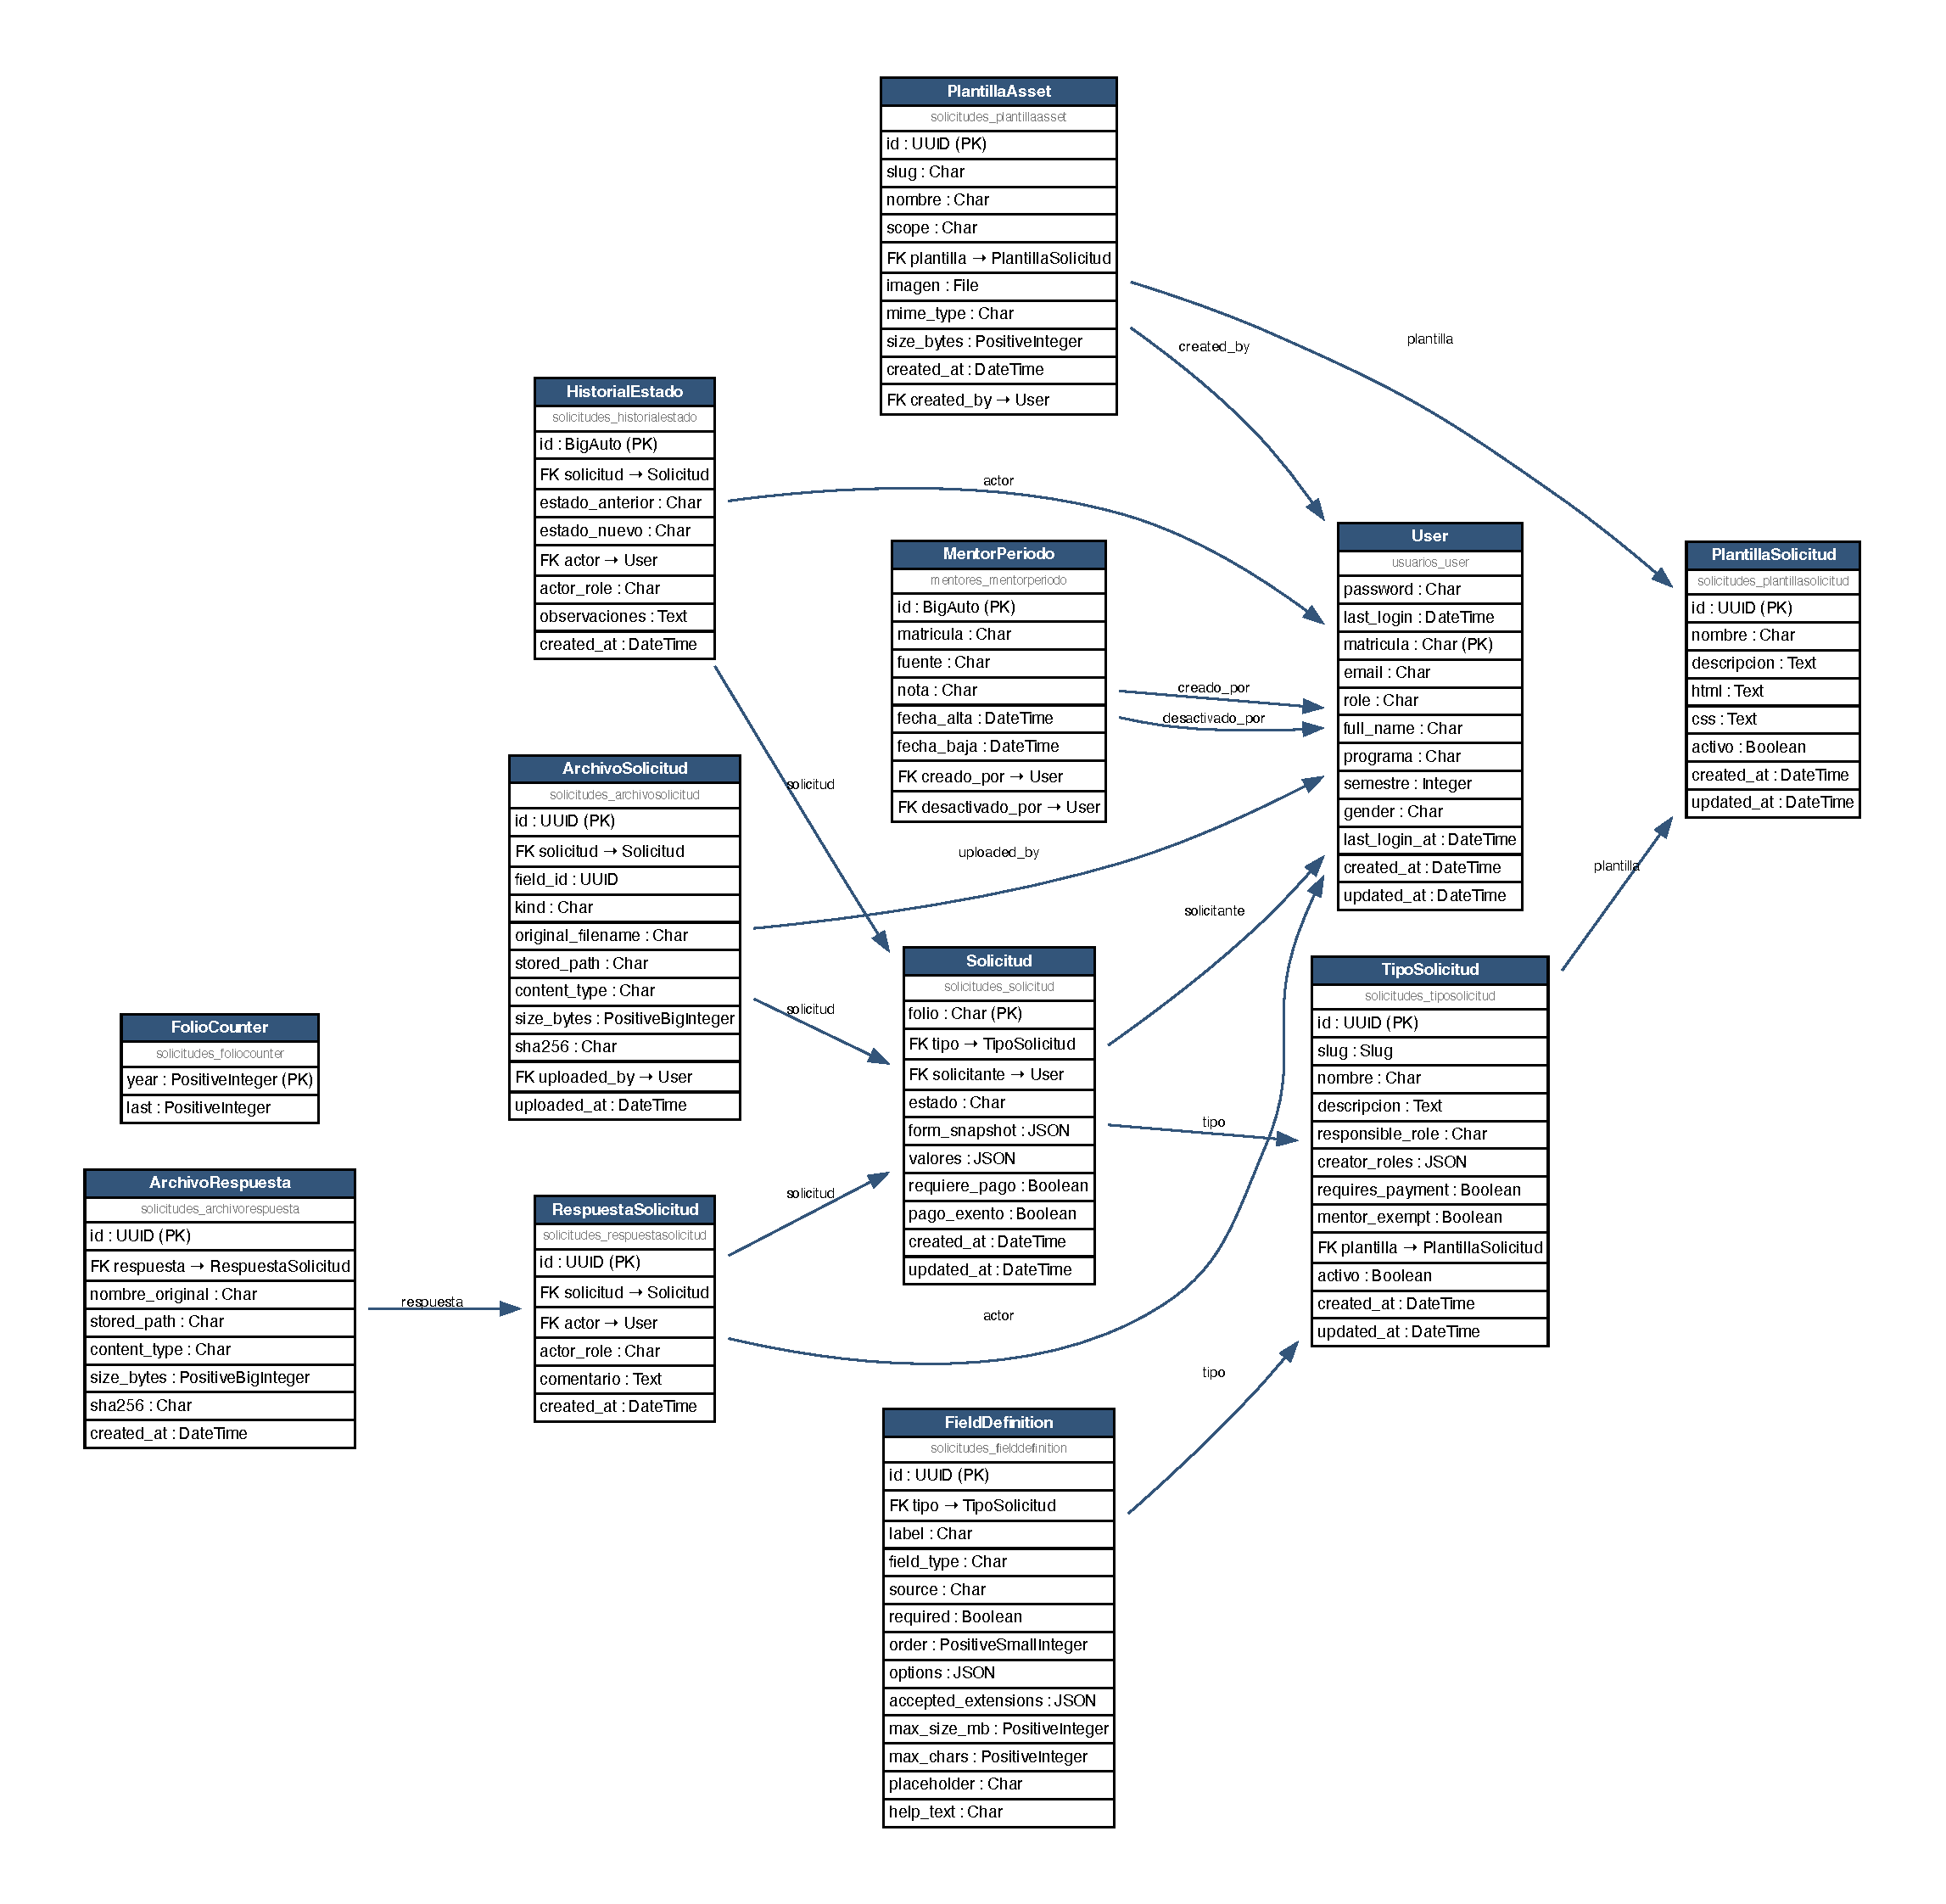
\includegraphics[width=\linewidth,height=0.9\textheight,keepaspectratio]{../esquema_bd_diagrama.pdf}
  \caption{Diagrama entidad-relación del Sistema de Solicitudes.}
  \label{fig:er}
\end{figure}
\end{landscape}

\chapter{Diccionario de datos}

Cada subsección documenta una entidad: su nombre de tabla física y la
descripción de cada columna (campo, tipo, si admite nulos, condición de llave y
descripción semántica). La abreviatura \textbf{PK} indica llave primaria y
\textbf{FK} llave foránea.

\section{User}

\textbf{Tabla:} \texttt{usuarios\_user}. Usuario del sistema, identificado por
su matrícula institucional. La autenticación es externa (proveedor de identidad
vía JWT); el modelo no emite tokens ni gestiona contraseñas, sólo cachea los
atributos de identidad provenientes del JWT y de SIGA para que las funciones
consumidoras los lean sin un segundo viaje.

\begin{longtable}{L{2.9cm} L{2.6cm} C{1.0cm} C{1.0cm} L{6.6cm}}
\toprule
\textbf{Campo} & \textbf{Tipo} & \textbf{Nulo} & \textbf{Llave} & \textbf{Descripción} \\
\midrule
\endhead
matricula & CharField(20) & No & PK & Matrícula institucional; identificador natural del usuario. \\
email & CharField(254) & No & --- & Correo electrónico (único). \\
role & CharField(32) & No & --- & Rol: ALUMNO, DOCENTE, CONTROL\_ESCOLAR, RESPONSABLE\_PROGRAMA o ADMIN. \\
full\_name & CharField(200) & No & --- & Nombre completo cacheado desde el JWT/SIGA. \\
programa & CharField(200) & No & --- & Programa educativo del usuario. \\
semestre & IntegerField & Sí & --- & Semestre actual (sólo aplica a alumnos). \\
gender & CharField(1) & No & --- & Código de género de SIGA: ``H'', ``M'' o vacío (sin información). \\
password & CharField(128) & No & --- & Heredado de Django; nunca se escribe (auth externa). \\
last\_login & DateTimeField & Sí & --- & Último acceso registrado por Django. \\
last\_login\_at & DateTimeField & Sí & --- & Último acceso registrado por la aplicación. \\
created\_at & DateTimeField & No & --- & Fecha de alta del registro. \\
updated\_at & DateTimeField & No & --- & Fecha de última actualización. \\
\bottomrule
\end{longtable}

\section{TipoSolicitud}

\textbf{Tabla:} \texttt{solicitudes\_tiposolicitud}. Entrada de catálogo que
describe una clase de solicitud: es la plantilla a partir de la cual se
levantan solicitudes. Lleva metadatos de enrutamiento (quién puede crearla y
quién la atiende), postura de pago, referencia a una plantilla PDF y una
bandera de baja lógica (\texttt{activo}); nunca se elimina físicamente una vez
que existe una solicitud asociada.

\begin{longtable}{L{2.9cm} L{2.6cm} C{1.0cm} C{1.0cm} L{6.6cm}}
\toprule
\textbf{Campo} & \textbf{Tipo} & \textbf{Nulo} & \textbf{Llave} & \textbf{Descripción} \\
\midrule
\endhead
id & UUIDField & No & PK & Identificador único. \\
slug & SlugField(80) & No & --- & Identificador legible único del tipo. \\
nombre & CharField(120) & No & --- & Nombre del tipo de solicitud. \\
descripcion & TextField & No & --- & Descripción del tipo. \\
responsible\_role & CharField(32) & No & --- & Rol responsable de atender las solicitudes de este tipo. \\
creator\_roles & JSONField & No & --- & Lista de roles autorizados para crear este tipo. \\
requires\_payment & BooleanField & No & --- & Indica si el tipo requiere pago. \\
mentor\_exempt & BooleanField & No & --- & Si los mentores quedan exentos del pago (sólo aplica con requires\_payment). \\
plantilla & FK $\rightarrow$ PlantillaSolicitud & Sí & FK & Plantilla PDF asociada (opcional). \\
activo & BooleanField & No & --- & Bandera de baja lógica (tombstone). \\
created\_at & DateTimeField & No & --- & Fecha de alta del registro. \\
updated\_at & DateTimeField & No & --- & Fecha de última actualización. \\
\bottomrule
\end{longtable}

\section{FieldDefinition}

\textbf{Tabla:} \texttt{solicitudes\_fielddefinition}. Define un campo tipado
del formulario dinámico de un \texttt{TipoSolicitud}. La fuente del valor
(\texttt{source}) indica si lo captura el alumno (\texttt{USER\_INPUT}) o si se
hidrata automáticamente desde los datos del usuario.

\begin{longtable}{L{2.9cm} L{2.6cm} C{1.0cm} C{1.0cm} L{6.6cm}}
\toprule
\textbf{Campo} & \textbf{Tipo} & \textbf{Nulo} & \textbf{Llave} & \textbf{Descripción} \\
\midrule
\endhead
id & UUIDField & No & PK & Identificador único. \\
tipo & FK $\rightarrow$ TipoSolicitud & No & FK & Tipo de solicitud al que pertenece el campo. \\
label & CharField(120) & No & --- & Etiqueta visible del campo. \\
field\_type & CharField(16) & No & --- & Tipo de control: TEXT, TEXTAREA, NUMBER, DATE, SELECT o FILE. \\
source & CharField(24) & No & --- & Origen del valor (USER\_INPUT o atributo del usuario). \\
required & BooleanField & No & --- & Indica si el campo es obligatorio. \\
order & PositiveSmallIntegerField & No & --- & Orden de presentación dentro del formulario. \\
options & JSONField & No & --- & Opciones para campos SELECT. \\
accepted\_extensions & JSONField & No & --- & Extensiones permitidas para campos FILE. \\
max\_size\_mb & PositiveIntegerField & No & --- & Tamaño máximo en MB para campos FILE (por defecto 10). \\
max\_chars & PositiveIntegerField & Sí & --- & Máximo de caracteres para TEXT/TEXTAREA (NULL usa el valor por defecto). \\
placeholder & CharField(200) & No & --- & Texto de marcador de posición. \\
help\_text & CharField(300) & No & --- & Texto de ayuda del campo. \\
\bottomrule
\end{longtable}

\section{Solicitud}

\textbf{Tabla:} \texttt{solicitudes\_solicitud}. Solicitud levantada; es una
instantánea del formulario de un \texttt{TipoSolicitud} al momento del alta. Se
identifica por su folio legible \texttt{SOL-AAAA-NNNNN}. La definición del
formulario que la produjo queda \emph{congelada} en \texttt{form\_snapshot}: las
ediciones posteriores al tipo no alteran lo originalmente enviado.

\begin{longtable}{L{2.9cm} L{2.6cm} C{1.0cm} C{1.0cm} L{6.6cm}}
\toprule
\textbf{Campo} & \textbf{Tipo} & \textbf{Nulo} & \textbf{Llave} & \textbf{Descripción} \\
\midrule
\endhead
folio & CharField(20) & No & PK & Folio legible (SOL-AAAA-NNNNN); identificador de negocio. \\
tipo & FK $\rightarrow$ TipoSolicitud & No & FK & Tipo de solicitud asociado. \\
solicitante & FK $\rightarrow$ User & No & FK & Usuario que levantó la solicitud. \\
estado & CharField(16) & No & --- & Estado: CREADA, EN\_PROCESO, FINALIZADA o CANCELADA. \\
form\_snapshot & JSONField & No & --- & Instantánea congelada de la definición del formulario al alta. \\
valores & JSONField & No & --- & Valores capturados (field\_id $\rightarrow$ valor primitivo). \\
requiere\_pago & BooleanField & No & --- & Pago requerido, capturado al alta. \\
pago\_exento & BooleanField & No & --- & Exención de pago resuelta al alta. \\
created\_at & DateTimeField & No & --- & Fecha de alta de la solicitud. \\
updated\_at & DateTimeField & No & --- & Fecha de última actualización. \\
\bottomrule
\end{longtable}

\section{HistorialEstado}

\textbf{Tabla:} \texttt{solicitudes\_historialestado}. Bitácora de
transiciones de estado por solicitud, sólo de adición (append-only). Cada
registro guarda el estado anterior (o \texttt{NULL} para el alta inicial
CREADA), el estado nuevo, el actor que disparó la transición, el rol del actor
en ese momento (instantánea) y observaciones opcionales.

\begin{longtable}{L{2.9cm} L{2.6cm} C{1.0cm} C{1.0cm} L{6.6cm}}
\toprule
\textbf{Campo} & \textbf{Tipo} & \textbf{Nulo} & \textbf{Llave} & \textbf{Descripción} \\
\midrule
\endhead
id & BigAutoField & No & PK & Identificador autoincremental. \\
solicitud & FK $\rightarrow$ Solicitud & No & FK & Solicitud a la que pertenece la entrada. \\
estado\_anterior & CharField(16) & Sí & --- & Estado previo (NULL sólo para el alta inicial CREADA). \\
estado\_nuevo & CharField(16) & No & --- & Estado resultante de la transición. \\
actor & FK $\rightarrow$ User & No & FK & Usuario que ejecutó la transición. \\
actor\_role & CharField(32) & No & --- & Rol del actor al momento de la transición (instantánea). \\
observaciones & TextField & No & --- & Observaciones opcionales del actor. \\
created\_at & DateTimeField & No & --- & Fecha y hora de la transición. \\
\bottomrule
\end{longtable}

\section{ArchivoSolicitud}

\textbf{Tabla:} \texttt{solicitudes\_archivosolicitud}. Registro índice de un
archivo adjunto a una solicitud. Guarda \emph{qué} se subió (nombre original,
tipo de contenido, tamaño, hash) y \emph{dónde} viven los bytes
(\texttt{stored\_path}, relativo a MEDIA\_ROOT). Distingue entre archivos de
formulario (\texttt{FORM}) y el comprobante de pago (\texttt{COMPROBANTE}).

\begin{longtable}{L{2.9cm} L{2.6cm} C{1.0cm} C{1.0cm} L{6.6cm}}
\toprule
\textbf{Campo} & \textbf{Tipo} & \textbf{Nulo} & \textbf{Llave} & \textbf{Descripción} \\
\midrule
\endhead
id & UUIDField & No & PK & Identificador único. \\
solicitud & FK $\rightarrow$ Solicitud & No & FK & Solicitud a la que pertenece el archivo. \\
field\_id & UUIDField & Sí & --- & ID del FieldDefinition (kind=FORM); NULL si es comprobante. No es FK real. \\
kind & CharField(16) & No & --- & Tipo de archivo: FORM o COMPROBANTE. \\
original\_filename & CharField(255) & No & --- & Nombre original del archivo. \\
stored\_path & CharField(500) & No & --- & Ruta de almacenamiento relativa a MEDIA\_ROOT. \\
content\_type & CharField(100) & No & --- & Tipo MIME del archivo. \\
size\_bytes & PositiveBigIntegerField & No & --- & Tamaño del archivo en bytes. \\
sha256 & CharField(64) & No & --- & Hash SHA-256 del contenido. \\
uploaded\_by & FK $\rightarrow$ User & No & FK & Usuario que subió el archivo. \\
uploaded\_at & DateTimeField & No & --- & Fecha y hora de la subida. \\
\bottomrule
\end{longtable}

\section{PlantillaSolicitud}

\textbf{Tabla:} \texttt{solicitudes\_plantillasolicitud}. Plantilla HTML/CSS
administrada para renderizar una solicitud como PDF. Es referenciada por
\texttt{TipoSolicitud.plantilla}. El cuerpo HTML usa sintaxis de plantilla
Django; los bytes del PDF no se almacenan: cada descarga se vuelve a renderizar
a partir de la fuente.

\begin{longtable}{L{2.9cm} L{2.6cm} C{1.0cm} C{1.0cm} L{6.6cm}}
\toprule
\textbf{Campo} & \textbf{Tipo} & \textbf{Nulo} & \textbf{Llave} & \textbf{Descripción} \\
\midrule
\endhead
id & UUIDField & No & PK & Identificador único. \\
nombre & CharField(120) & No & --- & Nombre de la plantilla. \\
descripcion & TextField & No & --- & Descripción de la plantilla. \\
html & TextField & No & --- & Cuerpo HTML con sintaxis de plantilla Django. \\
css & TextField & No & --- & Hoja de estilos asociada. \\
activo & BooleanField & No & --- & Indica si la plantilla está activa. \\
created\_at & DateTimeField & No & --- & Fecha de alta del registro. \\
updated\_at & DateTimeField & No & --- & Fecha de última actualización. \\
\bottomrule
\end{longtable}

\section{PlantillaAsset}

\textbf{Tabla:} \texttt{solicitudes\_plantillaasset}. Imagen subida por el
administrador para incrustar en las plantillas PDF. Tiene dos ámbitos
(\texttt{scope}): \texttt{global} (recursos institucionales disponibles para
toda plantilla) y \texttt{plantilla} (específicos de una sola plantilla). Las
plantillas referencian un asset por su \texttt{slug}.

\begin{longtable}{L{2.9cm} L{2.6cm} C{1.0cm} C{1.0cm} L{6.6cm}}
\toprule
\textbf{Campo} & \textbf{Tipo} & \textbf{Nulo} & \textbf{Llave} & \textbf{Descripción} \\
\midrule
\endhead
id & UUIDField & No & PK & Identificador único. \\
slug & CharField(64) & No & --- & Identificador legible referenciado desde la plantilla. \\
nombre & CharField(120) & No & --- & Nombre del recurso. \\
scope & CharField(10) & No & --- & Ámbito: global o plantilla. \\
plantilla & FK $\rightarrow$ PlantillaSolicitud & Sí & FK & Plantilla dueña (NULL cuando scope=global). \\
imagen & FileField(100) & No & --- & Ruta del archivo de imagen almacenado. \\
mime\_type & CharField(50) & No & --- & Tipo MIME de la imagen. \\
size\_bytes & PositiveIntegerField & No & --- & Tamaño del archivo en bytes. \\
created\_at & DateTimeField & No & --- & Fecha de alta del registro. \\
created\_by & FK $\rightarrow$ User & No & FK & Usuario que subió el recurso. \\
\bottomrule
\end{longtable}

\section{RespuestaSolicitud}

\textbf{Tabla:} \texttt{solicitudes\_respuestasolicitud}. Lote de respuesta
(archivos más comentario) cargado por el personal responsable durante el estado
EN\_PROCESO. Es de sólo adición a nivel de aplicación. Cada lote puede llevar de
0 a 10 archivos hijos (\texttt{ArchivoRespuesta}) y un comentario opcional.

\begin{longtable}{L{2.9cm} L{2.6cm} C{1.0cm} C{1.0cm} L{6.6cm}}
\toprule
\textbf{Campo} & \textbf{Tipo} & \textbf{Nulo} & \textbf{Llave} & \textbf{Descripción} \\
\midrule
\endhead
id & UUIDField & No & PK & Identificador único. \\
solicitud & FK $\rightarrow$ Solicitud & No & FK & Solicitud a la que responde el lote. \\
actor & FK $\rightarrow$ User & No & FK & Usuario que generó la respuesta. \\
actor\_role & CharField(32) & No & --- & Rol del actor al momento de responder (instantánea). \\
comentario & TextField & No & --- & Comentario opcional del lote. \\
created\_at & DateTimeField & No & --- & Fecha y hora de la respuesta. \\
\bottomrule
\end{longtable}

\section{ArchivoRespuesta}

\textbf{Tabla:} \texttt{solicitudes\_archivorespuesta}. Archivo almacenado
perteneciente a un lote \texttt{RespuestaSolicitud}.

\begin{longtable}{L{2.9cm} L{2.6cm} C{1.0cm} C{1.0cm} L{6.6cm}}
\toprule
\textbf{Campo} & \textbf{Tipo} & \textbf{Nulo} & \textbf{Llave} & \textbf{Descripción} \\
\midrule
\endhead
id & UUIDField & No & PK & Identificador único. \\
respuesta & FK $\rightarrow$ RespuestaSolicitud & No & FK & Lote de respuesta al que pertenece. \\
nombre\_original & CharField(255) & No & --- & Nombre original del archivo. \\
stored\_path & CharField(500) & No & --- & Ruta de almacenamiento relativa a MEDIA\_ROOT. \\
content\_type & CharField(120) & No & --- & Tipo MIME del archivo. \\
size\_bytes & PositiveBigIntegerField & No & --- & Tamaño del archivo en bytes. \\
sha256 & CharField(64) & No & --- & Hash SHA-256 del contenido. \\
created\_at & DateTimeField & No & --- & Fecha de alta del registro. \\
\bottomrule
\end{longtable}

\section{MentorPeriodo}

\textbf{Tabla:} \texttt{mentores\_mentorperiodo}. Catálogo de mentores
historizado por periodo (alta, baja): un registro por periodo de mentoría. La
reactivación abre un nuevo periodo (un nuevo registro) en lugar de sobrescribir
el anterior. Un índice único parcial impone ``a lo sumo un periodo abierto por
matrícula''.

\begin{longtable}{L{2.9cm} L{2.6cm} C{1.0cm} C{1.0cm} L{6.6cm}}
\toprule
\textbf{Campo} & \textbf{Tipo} & \textbf{Nulo} & \textbf{Llave} & \textbf{Descripción} \\
\midrule
\endhead
id & BigAutoField & No & PK & Identificador autoincremental. \\
matricula & CharField(20) & No & --- & Matrícula del mentor (indexada). \\
fuente & CharField(16) & No & --- & Origen del alta: MANUAL o CSV. \\
nota & CharField(200) & No & --- & Nota libre asociada al periodo. \\
fecha\_alta & DateTimeField & No & --- & Inicio del periodo de mentoría. \\
fecha\_baja & DateTimeField & Sí & --- & Fin del periodo (NULL = periodo activo). \\
creado\_por & FK $\rightarrow$ User & No & FK & Usuario que dio de alta el periodo. \\
desactivado\_por & FK $\rightarrow$ User & Sí & FK & Usuario que dio de baja el periodo (NULL si sigue activo). \\
\bottomrule
\end{longtable}

\section{FolioCounter}

\textbf{Tabla:} \texttt{solicitudes\_foliocounter}. Asignador de secuencia de
folios por año. El folio tiene forma \texttt{SOL-AAAA-NNNNN}; el componente
\texttt{NNNNN} se asigna bloqueando la fila del contador
(\texttt{SELECT \dots\ FOR UPDATE}) e incrementando \texttt{last}. Es la
estrategia portable entre PostgreSQL y SQLite.

\begin{longtable}{L{2.9cm} L{2.6cm} C{1.0cm} C{1.0cm} L{6.6cm}}
\toprule
\textbf{Campo} & \textbf{Tipo} & \textbf{Nulo} & \textbf{Llave} & \textbf{Descripción} \\
\midrule
\endhead
year & PositiveIntegerField & No & PK & Año de la secuencia. \\
last & PositiveIntegerField & No & --- & Último consecutivo asignado en el año. \\
\bottomrule
\end{longtable}

\chapter{Relaciones e integridad referencial}

\section{Llaves foráneas}

La Tabla~\ref{tab:fks} resume todas las relaciones de llave foránea, su
cardinalidad y la política de borrado (\texttt{on\_delete}) que define el
comportamiento ante la eliminación del registro referenciado.

\begin{longtable}{L{3.2cm} L{3.2cm} C{1.2cm} L{2.6cm} L{4.2cm}}
\caption{Llaves foráneas e integridad referencial.}
\label{tab:fks} \\
\toprule
\textbf{Origen (columna)} & \textbf{Destino} & \textbf{Card.} & \textbf{on\_delete} & \textbf{Semántica} \\
\midrule
\endhead
TipoSolicitud.plantilla & PlantillaSolicitud & N:1 & SET\_NULL & Al borrar la plantilla, el tipo queda sin plantilla. \\
FieldDefinition.tipo & TipoSolicitud & N:1 & CASCADE & Los campos se eliminan con su tipo. \\
Solicitud.tipo & TipoSolicitud & N:1 & PROTECT & No se puede borrar un tipo con solicitudes. \\
Solicitud.solicitante & User & N:1 & PROTECT & No se puede borrar un usuario con solicitudes. \\
HistorialEstado.solicitud & Solicitud & N:1 & CASCADE & La bitácora se elimina con su solicitud. \\
HistorialEstado.actor & User & N:1 & PROTECT & Protege la integridad de la auditoría. \\
ArchivoSolicitud.solicitud & Solicitud & N:1 & CASCADE & Los archivos se eliminan con su solicitud. \\
ArchivoSolicitud.uploaded\_by & User & N:1 & PROTECT & Protege la trazabilidad del autor. \\
PlantillaAsset.plantilla & PlantillaSolicitud & N:1 & CASCADE & Los assets de ámbito plantilla se eliminan con ella. \\
PlantillaAsset.created\_by & User & N:1 & PROTECT & Protege la trazabilidad del autor. \\
RespuestaSolicitud.solicitud & Solicitud & N:1 & CASCADE & Las respuestas se eliminan con su solicitud. \\
RespuestaSolicitud.actor & User & N:1 & PROTECT & Protege la trazabilidad del autor. \\
ArchivoRespuesta.respuesta & RespuestaSolicitud & N:1 & CASCADE & Los archivos se eliminan con su lote de respuesta. \\
MentorPeriodo.creado\_por & User & N:1 & PROTECT & Protege la trazabilidad del autor del alta. \\
MentorPeriodo.desactivado\_por & User & N:1 & PROTECT & Protege la trazabilidad del autor de la baja. \\
\bottomrule
\end{longtable}

\noindent\textbf{Referencia lógica sin FK.} \texttt{ArchivoSolicitud.field\_id}
referencia conceptualmente a \texttt{FieldDefinition.id} cuando
\texttt, pero \emph{no} es una llave foránea real: el formulario está
congelado en la solicitud (\texttt{form\_snapshot}) y la definición de campo
viva puede editarse o borrarse después. De forma análoga,
\texttt{MentorPeriodo.matricula} se relaciona por valor con
\texttt{User.matricula} sin imponer una FK.

\section{Restricciones únicas y de verificación}

\begin{itemize}[leftmargin=1.4em]
  \item \textbf{User.email} --- único en toda la tabla.
  \item \textbf{TipoSolicitud.slug} --- único en toda la tabla.
  \item \textbf{FieldDefinition} \texttt{(tipo, order)} ---
        \texttt{unique\_field\_order\_per\_tipo}: no se repite el orden de
        campos dentro de un mismo tipo.
  \item \textbf{ArchivoSolicitud} \texttt{(solicitud, field\_id)} con
        \texttt --- \texttt{archivo\_unique\_per\_field}: un solo
        archivo de formulario por campo de la solicitud (índice parcial).
  \item \textbf{ArchivoSolicitud} \texttt{(solicitud)} con
        \texttt --- \texttt{archivo\_unique\_comprobante}: un
        solo comprobante de pago por solicitud (índice parcial).
  \item \textbf{PlantillaAsset} \texttt{(slug)} con \texttt{scope=global} ---
        \texttt{unique\_global\_asset\_slug}: slug único entre los assets
        globales (índice parcial).
  \item \textbf{PlantillaAsset} \texttt{(plantilla, slug)} con
        \texttt{scope=plantilla} --- \texttt{unique\_plantilla\_asset\_slug}:
        slug único por plantilla (índice parcial).
  \item \textbf{PlantillaAsset} --- \texttt{plantilla\_asset\_scope\_consistency}
        (CHECK): coherencia entre ámbito y plantilla (global $\Rightarrow$
        plantilla nula; plantilla $\Rightarrow$ plantilla no nula).
  \item \textbf{MentorPeriodo} \texttt{(matricula)} con
        \texttt{fecha\_baja IS NULL} ---
        \texttt{unique\_active\_period\_per\_matricula}: a lo sumo un periodo de
        mentoría activo por matrícula (índice parcial; requiere PostgreSQL).
\end{itemize}

\section{Índices de consulta}

Además de los índices de llave primaria y de las restricciones únicas, el
esquema define índices secundarios para acelerar las consultas más frecuentes:

\begin{itemize}[leftmargin=1.4em]
  \item \textbf{TipoSolicitud} --- \texttt{(activo, responsible\_role)}.
  \item \textbf{Solicitud} --- \texttt{(solicitante, -created\_at)},
        \texttt{(estado, -created\_at)} y \texttt{(tipo, estado)}.
  \item \textbf{HistorialEstado} --- \texttt{(solicitud, -created\_at)}.
  \item \textbf{ArchivoSolicitud} --- \texttt{(solicitud, kind)}.
  \item \textbf{PlantillaSolicitud} --- \texttt{(activo, nombre)}.
  \item \textbf{RespuestaSolicitud} --- \texttt{(solicitud, created\_at)}.
  \item \textbf{ArchivoRespuesta} --- \texttt{(respuesta, created\_at)}.
  \item \textbf{MentorPeriodo} --- \texttt{(matricula, fecha\_baja)} y un índice
        simple sobre \texttt{matricula}.
\end{itemize}

\end{document}
